%----------------------------------------------------------------------------------------
%	PACKAGES AND OTHER DOCUMENT CONFIGURATIONS
%----------------------------------------------------------------------------------------

\documentclass[paper=a4, fontsize=11pt]{scrartcl} % A4 paper and 11pt font size

% ---- Entrada y salida de texto -----

\usepackage[T1]{fontenc} % Use 8-bit encoding that has 256 glyphs
\usepackage[utf8]{inputenc}
%\usepackage{fourier} % Use the Adobe Utopia font for the document - comment this line to return to the LaTeX default

% ---- Idioma --------

\usepackage[spanish, es-tabla]{babel} % Selecciona el español para palabras introducidas automáticamente, p.ej. "septiembre" en la fecha y especifica que se use la palabra Tabla en vez de Cuadro

% ---- Otros paquetes ----
\usepackage{csquotes} %Para permitir el uso de comillas Quotes https://tex.stackexchange.com/questions/36812/isnt-there-any-other-way-of-doing-double-quotes-in-latex-besides
\usepackage[hyphens]{url} % ,href} %para incluir URLs e hipervínculos dentro del texto (aunque hay que instalar href)
\usepackage{hyperref}
\usepackage{color}
\usepackage{graphics,graphicx, floatrow} %para incluir imágenes y notas en las imágenes
\usepackage{graphics,graphicx, float} %para incluir imágenes y colocarlas

\graphicspath {{./img/}}

\usepackage{listings}  %para introducir comandos

\lstdefinestyle{mybash}
{basicstyle=\ttfamily,
  showstringspaces=false,
  commentstyle=\color{red},
  keywordstyle=\color{blue},
  language=bash,
  alsoletter=/,
  basicstyle=\footnotesize,
  numbers=left,
  stepnumber=1,
  showstringspaces=false,
  tabsize=1,
  breaklines=true,
  breakatwhitespace=false,
}
\lstdefinestyle{mysql}
{basicstyle=\ttfamily,
  showstringspaces=false,
  commentstyle=\color{red},
  keywordstyle=\color{blue},
  language=sql,
  basicstyle=\footnotesize,
  numbers=left,
  stepnumber=1,
  showstringspaces=false,
  tabsize=1,
  breaklines=true,
  breakatwhitespace=false,
}


% Para hacer tablas comlejas
%\usepackage{multirow}
%\usepackage{threeparttable}

%\usepackage{sectsty} % Allows customizing section commands
%\allsectionsfont{\centering \normalfont\scshape} % Make all sections centered, the default font and small caps

\usepackage{fancyhdr} % Custom headers and footers
\pagestyle{fancyplain} % Makes all pages in the document conform to the custom headers and footers
\fancyhead{} % No page header - if you want one, create it in the same way as the footers below
\fancyfoot[L]{} % Empty left footer
\fancyfoot[C]{} % Empty center footer
\fancyfoot[R]{\thepage} % Page numbering for right footer
\renewcommand{\headrulewidth}{0pt} % Remove header underlines
\renewcommand{\footrulewidth}{0pt} % Remove footer underlines
\setlength{\headheight}{13.6pt} % Customize the height of the header

\setlength\parindent{0pt} % Removes all indentation from paragraphs - comment this line for an assignment with lots of text

\newcommand{\horrule}[1]{\rule{\linewidth}{#1}} % Create horizontal rule command with 1 argument of height


%----------------------------------------------------------------------------------------
%	TÍTULO Y DATOS DEL ALUMNO
%----------------------------------------------------------------------------------------
\graphicspath{ {img/} }

\title{
\normalfont \normalsize

\includegraphics[width=6cm,height=6cm]{logo}\\
\textsc{\textbf{Bootcamp Especialidad GNU/Linux (2023)}} \\ [25pt] % Your university, school and/or department name(s)
\horrule{0.5pt} \\[0.4cm] % Thin top horizontal rule
\huge Lab 05 - Monitorización, análisis y almacenamiento de registros. \\ % The assignment title
\horrule{2pt} \\[0.5cm] % Thick bottom horizontal rule
}


%https://es.overleaf.com/learn/latex/Inserting_Images
%Ruta relativa de   imagenes

\author{Pedro Antonio Mayorgas Parejo} % Nombre y apellidos

\date{\normalsize\today} % Incluye la fecha actual

%----------------------------------------------------------------------------------------
% DOCUMENTO
%----------------------------------------------------------------------------------------

\begin{document}

\maketitle % Muestra el Título

\newpage %inserta un salto de página

\tableofcontents % para generar el índice de contenidos

\newpage

%----------------------------------------------------------------------------------------
%	Cuestión 1
%----------------------------------------------------------------------------------------

\section{Instalación y configuración de Fail2ban}

Para instalar el servicio, debemos ejecutar el siguiente comando:

\begin{lstlisting}[style=mybash]
sudo apt install fail2ban
\end{lstlisting}

\begin{figure}[H]
	\centering
	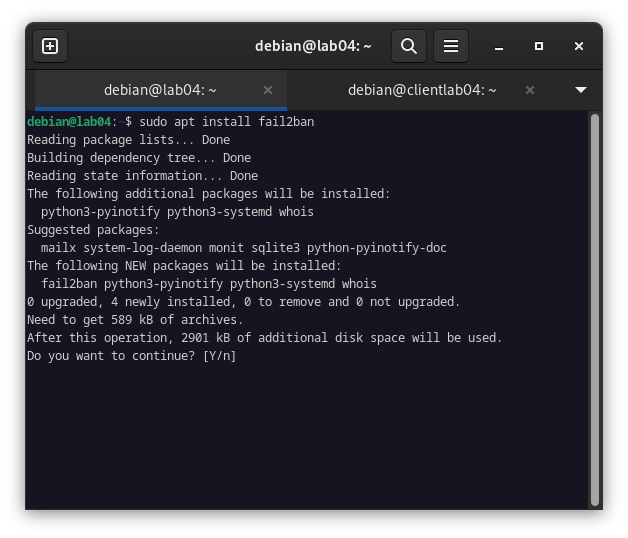
\includegraphics[scale=0.40]{00}
	\caption{Instalación de fail2ban.}
\end{figure}

Las configuraciones realizadas en \textbf{/etc/fail2ban/jail.conf}, son las siguientes:

\begin{itemize}
\item Se habilita un incremento de la expulsión (ban).
\item Se habilita una expulsión de 10 minutos y el número de intentos antes de ban.
\item El resto de servicios deben ser eliminado de la lista de observación de fail2ban para minimizar los fallos.
\item Se configura el backend de log para systemd, porque en sistemas GNU/Linux con systemd no tienen los clásicos ficheros en texto plano configurados.
\end{itemize}

\begin{figure}[H]
	\centering
	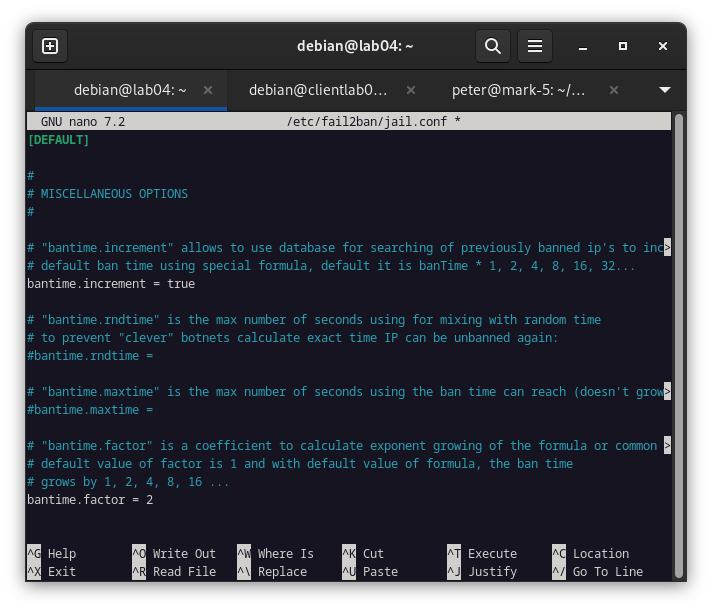
\includegraphics[scale=0.40]{01}
	\caption{Configuración del incremento de la expulsión.}
\end{figure}

\begin{figure}[H]
	\centering
	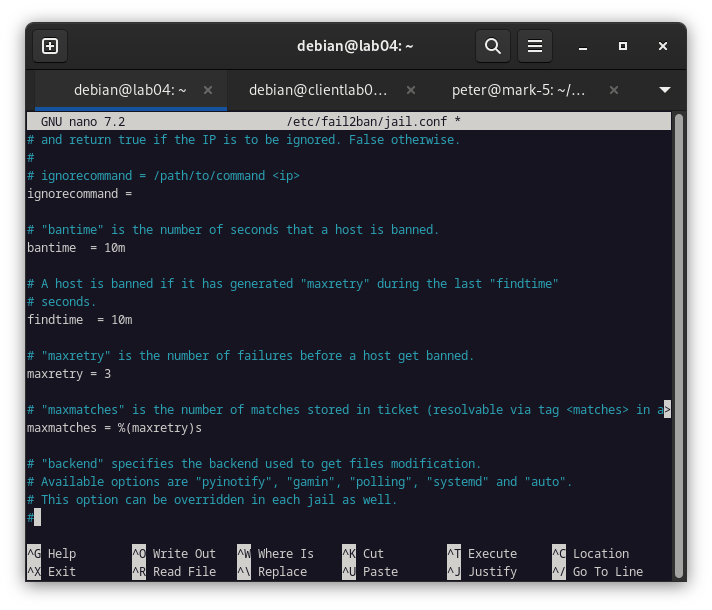
\includegraphics[scale=0.40]{02}
	\caption{Configuración de los intentos.}
\end{figure}


\begin{figure}[H]
	\centering
	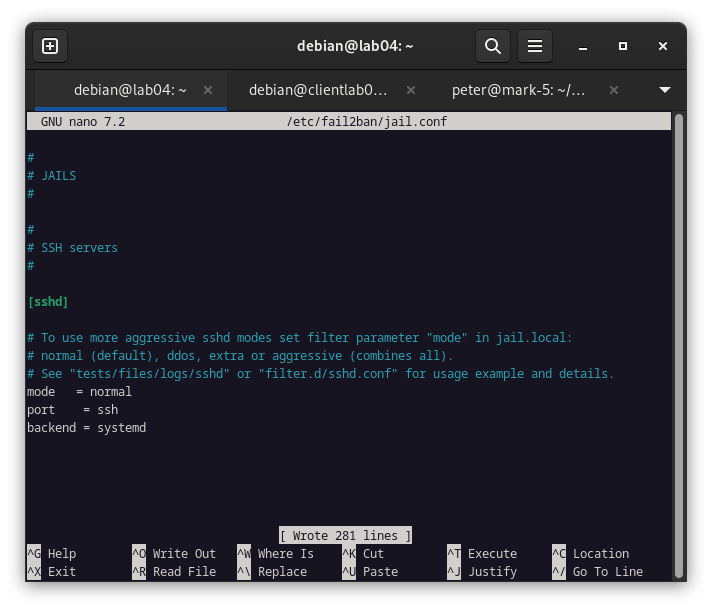
\includegraphics[scale=0.40]{04}
	\caption{Configuración de servicio sshd y backend.}
\end{figure}

Por último reiniciamos el servicio para aplicar los cambios y comprobar que funcionan correctamente con los siguientes comandos:

\begin{lstlisting}[style=mybash]
sudo systemctl restart fail2ban.service
sudo systemctl status fail2ban.service 
\end{lstlisting}

\begin{figure}[H]
	\centering
	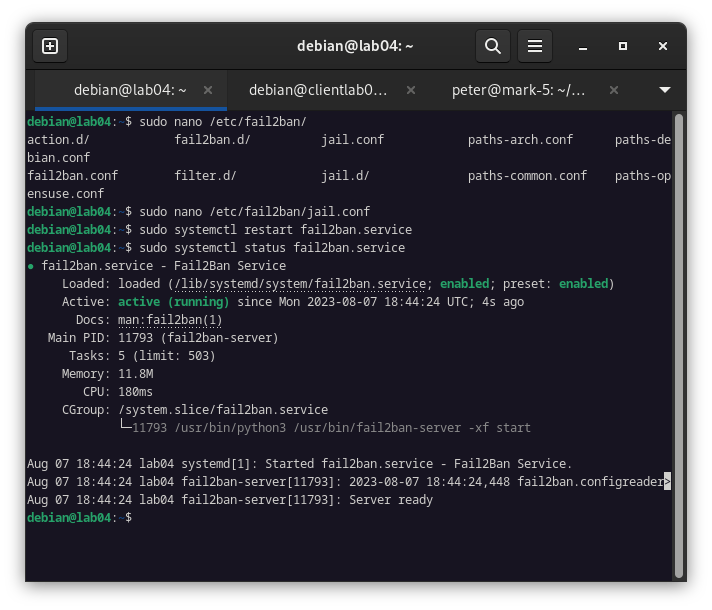
\includegraphics[scale=0.40]{05}
	\caption{Aplicando los cambios a fail2ban.}
\end{figure}

\newpage
\section{Probando fail2ban}

Ahora con un cliente que no tenga clave pública probamos que efectivamente se aplique el fail2ban y mostramos el log. Primero tenemos que habilitar el acceso por contraseña, ya que si lo hacemos por clave pública solo, fail2ban no salta, es decir porque está protegido el sshd. En este caso habilitamos la opción de contraseña para el usuario pedrolab04, para hacer intentos por contraseña.

\begin{figure}[H]
	\centering
	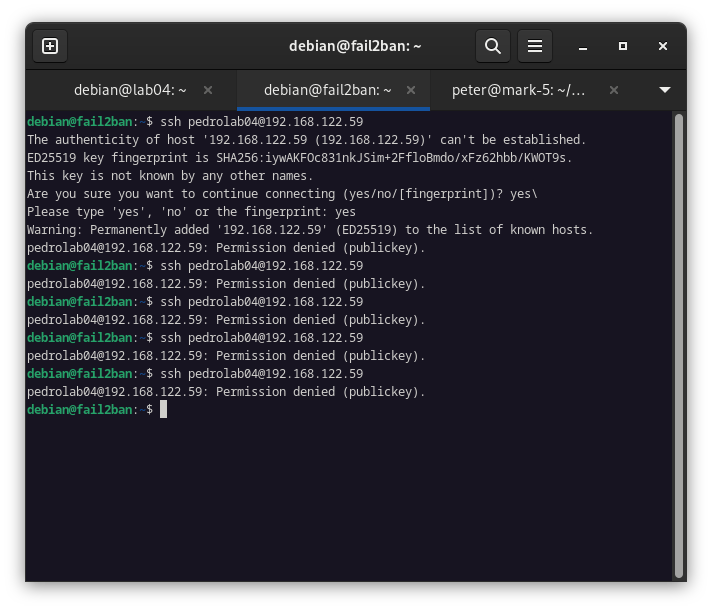
\includegraphics[scale=0.40]{06}
	\caption{Si aplicamos solo clave pública no funcionará fail2ban, no le hace falta.}
\end{figure}

El ban por IP se puede comprobar cuando intentamos realizar una conexión que en vez de preguntarnos por la contraseña nos indica que se ha rechazado la conexión. Es decir el siguiente mensaje:
\vspace{5mm}

\textbf{ssh: connect to host 192.168.122.59 port 22: Connection refused}
\begin{figure}[H]
	\centering
	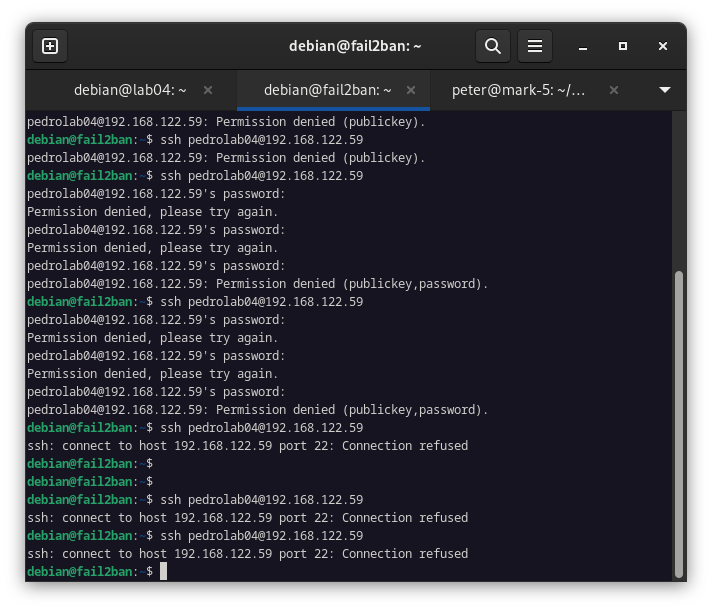
\includegraphics[scale=0.40]{07}
	\caption{Una vez aplicado la autenticación por contraseña al tercer intento se banea por IP.}
\end{figure}

Una vez que el ban se aplica se puede ver el estado del ban en un comando de fail2ban.

\begin{lstlisting}[style=mybash]
sudo fail2ban-client status sshd
\end{lstlisting}

\begin{figure}[H]
	\centering
	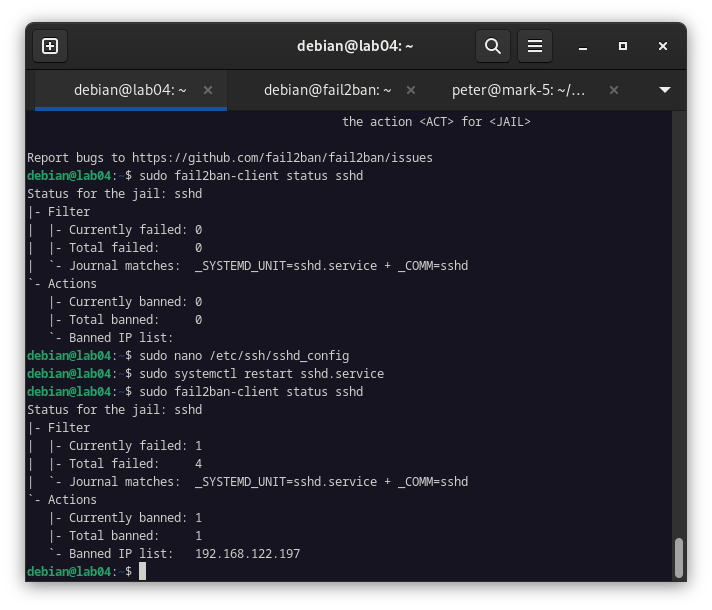
\includegraphics[scale=0.40]{08}
	\caption{Podemos ver el ban en el comando y la IP.}
\end{figure}

Para hacer unban al cliente sin esperar, tenemos que introducir el siguiente comando:

\begin{lstlisting}[style=mybash]
sudo fail2ban-client unban 192.168.122.197
\end{lstlisting}

\begin{figure}[H]
	\centering
	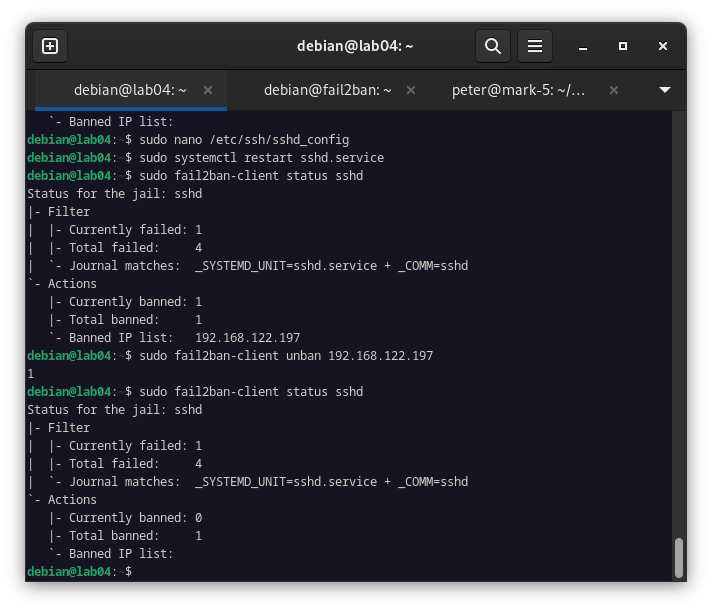
\includegraphics[scale=0.40]{09}
	\caption{Aplicando el unban.}
\end{figure}

\begin{figure}[H]
	\centering
	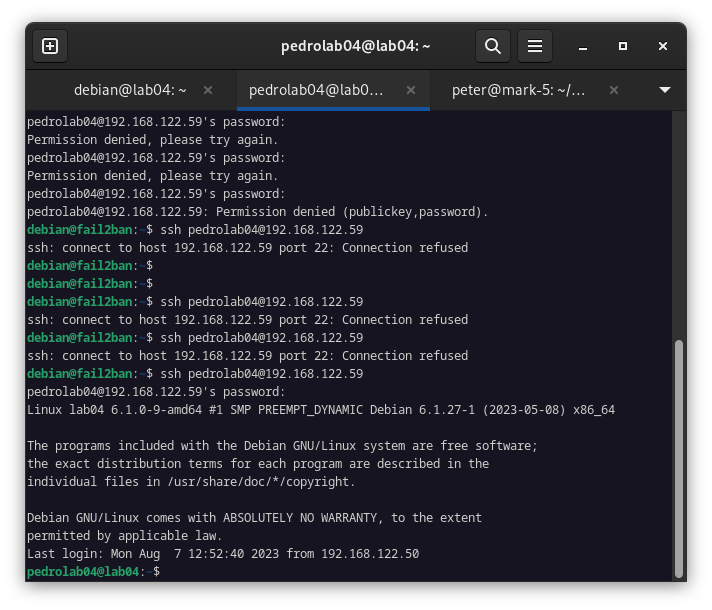
\includegraphics[scale=0.40]{10}
	\caption{El cliente después de estar baneado puede autenticarse correctamente.}
\end{figure}

Fuentes \textbf{https://itslinuxfoss.com/unban-ip-fail2ban/} \textbf{https://www.cyberciti.biz/faq/how-to-protect-ssh-with-fail2ban-on-centos-8/}
% \vspace{5mm}


% \begin{lstlisting}[style=mybash]
%     # Para una base de datos concreta
%     mysqldump --user=tiendabd --password=password --databases tiendabd --add-drop-database --add-drop-table [--replace] --host=127.0.0.1 --result-file=dump.sql
% \end{lstlisting}



%\begin{figure}[H]
%	\centering
%	\includegraphics[scale=0.40]{cuestion_1_1}
%	\caption{Se puede ver que al no haber un fallo grave, el sistema lo nota como que sigue funcionando pero en un estado degradado.}
%\end{figure}

%\newpage

%Se pueden hacer include en latex
%\newpage

\section{Section}

\subsection{Subseccion}

\subsubsection{Subseccion}



%-------Bibliografia-----------------------------

%\newpage
\section{Bibliografía}

% Ejemplo
\footnote{Administración de mdadm - Por Red Hat}
\textcolor{blue}{\url{https://access.redhat.com/documentation/en-us/red_hat_enterprise_linux/8/html/managing_storage_devices/managing-raid_managing-storage-devices#monitoring-raid_managing-raid}}



\end{document}
